%Poster do trabalho de conclusao de curso 

\documentclass[final]{beamer}
\mode<presentation>{\usetheme{azul}}
\usepackage{graphicx}
\usepackage{epstopdf}
\usepackage{subfigure}

\usepackage[brazil]{babel}
\usepackage[utf8]{inputenc}
\usepackage{ragged2e} 

\usepackage[T1]{fontenc}
\usepackage[justification=centering]{caption}


\usepackage{amsmath,amsthm, amssymb, latexsym}
\usepackage[orientation=portrait,size=a2,scale=1.4]{beamerposter}
\usepackage[ruled]{algorithm2e}

\usepackage{snapshot} % will write a .dep file with all dependencies, allows for easy bundling

\DeclareMathSizes{17.42}{15}{14}{10}  % Math text size

%%%%%%%%%%%%%%%%%%%%%%%%%%%%%%%%
%%  MACROS %%%%%%%%%%%%%%%%%%%%%
\usepackage{xspace}
\newcommand{\pixel}{\emph{pixel}\xspace}
\newcommand{\pixels}{\emph{pixels}\xspace}
\newcommand{\voxel}{\emph{voxel}\xspace}
\newcommand{\voxels}{\emph{voxels}\xspace}


\listfiles
%%%%%%%%%%%%%%%%%%%%%%%%%%%%%%%%%%%%%%%%%%%%%%%%%%%%%%%%%%%%%%%%%%%%%%%%%%%%%%%%%%%%%%
\title{\huge Aplicando o Arcabouço OpenTuner em Jogos Digitais}

\author{Renan Teruo Carneiro, Vitor Cerqueira Santos <renantc@linux.ime.usp.br varyag@linux.ime.usp.br>, Orientador: Alfredo Goldman <gold@ime.usp.br>}
\institute[Universidade de São Paulo] % (optional, but mostly needed)
{
  Instituto de Matemática e Estatística, Universidade de São Paulo - Trabalho
  de Conclusão de Curso
}


\date[Novembro 2015]{Novembro, 2015}
%%%%%%%%%%%%%%%%%%%%%%%%%%%%%%%%%%%%%%%%%%%%%%%%%%%%%%%%%%%%%%%%%%%%%%%%%%%%%%%%%%%%%%
\newlength{\columnheight}
\setlength{\columnheight}{65cm}
%%%%%%%%%%%%%%%%%%%%%%%%%%%%%%%%%%%%%%%%%%%%%%%%%%%%%%%%%%%%%%%%%%%%%%%%%%%%%%%%%%%%%%
\begin{document}
\begin{frame}
  \begin{columns}
    % ---------------------------------------------------------%
    % Set up a column 
    \begin{column}{.5\textwidth}
      \begin{beamercolorbox}[center,wd=\textwidth]{postercolumn}
        \begin{minipage}[T]{.95\textwidth} % tweaks the width, makes a new \textwidth
          \parbox[t][\columnheight]{\textwidth}{ % must be some better way to set the the height, width and textwidth simultaneously
            % Since all columns are the same length, it is all nice and tidy.  You have to get the height empirically
            % ---------------------------------------------------------%
            % fill each column with content            
            
            \vspace*{0.8cm}
            
            \begin{block}{Introdução}
            \justifying
                Neste trabalho são exploradas possíveis aplicações do conceito de Autotuning, ou Ajuste Fino sobre jogos digitais. 
                                
                \vspace*{0.15cm}
                
                O autotuning parte da proposta de automatizar o processo de otimização de um programa, alterando seus parâmetros ou algoritmos de solução. Um sistema que realiza essa ação é comumente chamado de tuner, e ele pode funcionar de várias maneiras; o que ele faz, no entanto, é testar diversas configurações diferentes de parâmetros ou algoritmos, e escolher quais destas obtêm o melhor desempenho esperado para o programa, seja este um resultado mais favorável, ou um menor tempo de execução.
                
                \vspace*{0.15cm}
                
                Os possíveis usos e aplicações de um tuner no campo de jogos digitais são diversos, desde a criação de ferramentas externas para os jogadores que querem por exemplo, conseguir o máximo de seus pontos em um jogo, até possíveis implementações de meta-ferramentas de análise do jogo a nível de desenvolvimento.
                
                \vspace*{0.15cm}
                
                Para este trabalho, foi utilizado o OpenTuner, que é um arcabouço de ajuste fino focado em realizar otimização de parâmetros, analisando os resultados gerados pelo programa a ser ajustado e criando um espaço de busca com estes. Junto a esta ferramenta, foi escolhido como base para os testes, o jogo OpenTTD.
                
                \vspace*{0.15cm}
                
                O OpenTTD é um simulador de gerência de uma empresa de transportes, onde se é possível construir e controlar rotas de entrega, linhas de trem, entre outros meios de transporte. O jogo pode rodar inteligências artificiais que controlam outras empresas, e o autotuning foi feito sobre estas.

%                \textbf{AAAAAAAAAAAAAAAAAAA}
                
%                \vspace*{0.2cm}
            \end{block}
            
            \vspace*{0.2cm}

            \begin{block}{Objetivos}
              \justifying
              \begin{itemize}
                \item Verificar a viabilidade de aplicação de técnicas de autotuning sobre jogos digitais 
                
                \vspace*{0.4cm}
                
                \item Implementar um tuner aplicado a um jogo.
                
                \vspace*{0.4cm}
                
                \item Verificar o quanto um tuner pode afetar o desempenho de um aspecto do jogo 
              \end{itemize}
              \vspace*{0.2cm} 
            \end{block}
            
            \vspace*{0.2cm}

            \begin{block}{O OpenTuner}
            \justifying
                OpenTuner é um arcabouço para a implementação de sistemas de otimização e autotuning de programas. Utilizando um conjunto de técnicas empíricas de busca, o OpenTuner gera e testa combinações de parâmetros de configuração para um determinado programa, que podem representar por exemplo, escolhas algorítmicas. 
                
                \vspace*{0.2cm}
                
                O OpenTuner realiza a ação de otimização via um conjunto de métodos. O módulo de medição aceita resultados desejados na sua entrada, e executa o programa tentando chegar neles. Ao final da execução, os resultados observados são devolvidos para o módulo de otimização, que cria o espaço de busca do problema com estes resultados, e o navega criando novas parametrizações de resultados desejados, que são enviados novamente ao módulo de medição.
                
                \vspace*{0.4cm} 
                
                
                \begin{figure}[h]
                  \fbox{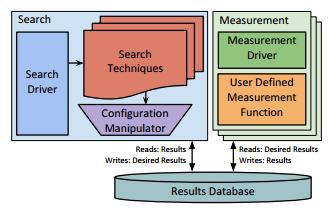
\includegraphics[width=0.4\textwidth]{OpenTuner.png}}
                  \caption{Método de funcionamento do OpenTuner.
                    Fonte: Ansel, Jason, et al, Opentuner: An extensible framework for program autotuning}
                \end{figure}
                
                \vspace*{0.2cm} 
                
                A decisão foi feita para aplicar o OpenTuner em algum projeto já existente, neste caso um jogo. A ideia básica é que podemos usar o OpenTuner para otimizar um conjunto de parâmetros dentro do jogo, para ajudar o jogador a ter um planejamento, ou como uma metaferramenta de auxílio.
                               
                \vspace*{0.2cm} 
            \end{block}
                        
            \vspace*{0.2cm}
          }
        \end{minipage}
      \end{beamercolorbox}
    \end{column}
    % ---------------------------------------------------------%
    % end the column

    % ---------------------------------------------------------%
    % Set up a column 
    \begin{column}{.5\textwidth}
      \begin{beamercolorbox}[center,wd=\textwidth]{postercolumn}
        \begin{minipage}[T]{.95\textwidth} % tweaks the width, makes a new \textwidth
          \parbox[t][\columnheight]{\textwidth}{ % must be some better way to set the the height, width and textwidth simultaneously
            % Since all columns are the same length, it is all nice and tidy.  You have to get the height empirically
            % ---------------------------------------------------------%
            % fill each column with content
            
            \vspace*{0.8cm}
            
            \begin{block}{OpenTTD}
                O Jogo
                \begin{itemize}
                  \item Simulador de gerência de uma empresa de transportes.
                  \item Pode-se comprar, vender e construir veículos e linhas de transporte, como trens.
                  \item Possui modo para vários jogadores, e suporta inteligências artificiais.
                \end{itemize}
                
                \vspace*{0.5cm}
                Para fazer os testes do tuner, foi buscada uma maneira de rodar e avaliar o desempenho de inteligências artificiais no ambiente do jogo.
                \begin{itemize}
                  \item Foi escolhida uma IA chamada ChooChoo, especializada no gerenciamento e construção de linhas de trem.
                  \item Foi decidido que o tuner tentaria otimizar os parâmetros da função de pathfinding da AI, como uma maneira de avaliar o impacto de tais mudanças.
                \end{itemize}  
                         
                \vspace*{0,5cm}
                
                A execução dos testes consiste em iniciar um servidor do jogo, inicializar uma IA
                
                \vspace*{0.2cm} 
            \end{block}

            \vspace*{0.2cm} 
            
            \begin{block}{Resultados}
              \justifying 
                O Tuner
                
                \vspace*{0.2cm} 
                
                Composto de três partes:
                \begin{itemize}
                	\item O construtor gera os arquivos a serem alterados para os testes e os passa para o tuner
                	\item O handler organiza e trata a saída do programa, comunicando-se com o tuner
                	\item O tuner então executa os testes em um servidor de jogo, carregando os arquivos de IA modificados, e colhendo seus resultados
                	\item Baseado nestes resultados, os novos parâmetros são gerados, e as informações necessárias para preparar os novos arquivos de teste são passadas para o construtor
                \end{itemize}
                
                \begin{figure}[htp]
                  \centering
                   \fbox{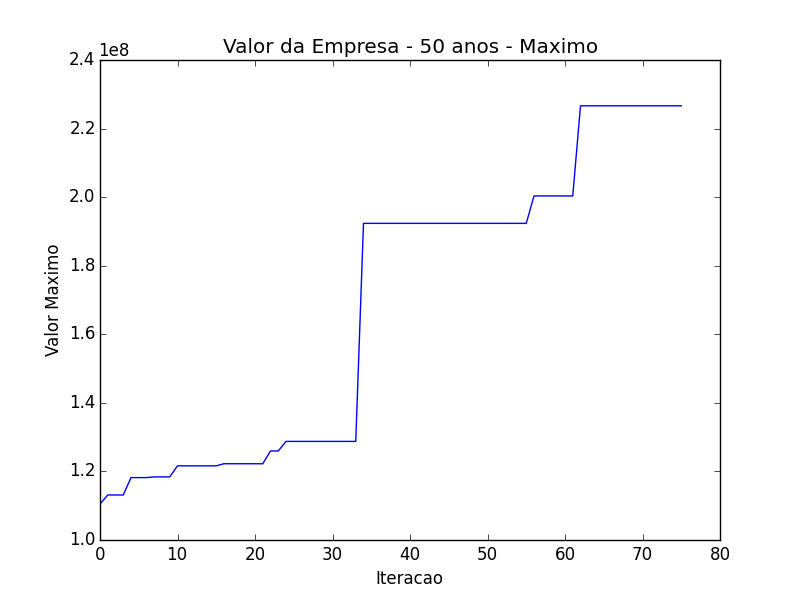
\includegraphics[width=0.6\textwidth]{value-50yrs-best.png}}
                  \caption{Teste com duração de 50 anos dentro do jogo}
                \end{figure}
                
                \vspace*{0.4cm}
                
                Resultados obtidos com esse exemplo incluem:
                \begin{itemize}
                  \item Funciona! O tuner consegue aumentar gradativamente o valor da empresa em testes subsequentes.
                  \item Mesmo otimizando um conjunto de parâmetros aparentemente não relacionado, os custos do algoritmo de pathfinding de construção de ferrovias.
                  \item Outros valores também foram avaliados, como o lucro final e o valor de caixa ao final do semestre, e também foram observadas melhoras.
                  \item Ainda não é possível realizar testes em paralelo com o OpenTuner, o que causa uma geração mais lenta de resultados, e um crescimento mais lento do espaço de busca do algoritmo.
                \end{itemize}
                
                \vspace*{0.2cm}
            \end{block}
            
%            \vspace*{0.2cm} 
%            \begin{block}{Trabalhos Futuros}
%                Durante o desenvolvimento do tuner, 
%                
%                \begin{itemize}
%                  \item 
%                  \item 
%                 
%                \end{itemize}
%                
%                \vspace*{0.2cm} 
%                
%            \end{block}
            
            \vspace*{0.2cm} 
            
            \begin{block}{Referências}
              \small
                \begin{itemize}
                    \item Ansel, Jason, et al. "Opentuner: An extensible framework for program autotuning." Proceedings of the 23rd international conference on Parallel architectures and compilation. ACM, 2014.
                \end{itemize}
                \vspace*{0.2cm} 
            \end{block}
            \vfill
          }
        \end{minipage}
      \end{beamercolorbox}
    \end{column}
    % ---------------------------------------------------------%
    % end the column


  \end{columns}
\end{frame}

\end{document}


%%%%%%%%%%%%%%%%%%%%%%%%%%%%%%%%%%%%%%%%%%%%%%%%%%%%%%%%%%%%%%%%%%%%%%%%%%%%%%%%%%%%%%%%%%%%%%%%%%%%
%%% Local Variables: 
%%% mode: latex
%%% TeX-PDF-mode: t
%%% End:
